\documentclass{article}

\usepackage{amsmath}
\usepackage{listings}
\usepackage{graphicx}
\usepackage{xcolor}

\definecolor{codegreen}{rgb}{0,0.6,0}
\definecolor{codegray}{rgb}{0.5,0.5,0.5}
\definecolor{codepurple}{rgb}{0.58,0,0.82}
\definecolor{backcolour}{rgb}{0.95,0.95,0.92}

\lstdefinestyle{mystyle}{
    backgroundcolor=\color{backcolour},   
    commentstyle=\color{codegreen},
    keywordstyle=\color{magenta},
    numberstyle=\tiny\color{codegray},
    stringstyle=\color{codepurple},
    basicstyle=\ttfamily\footnotesize,
    breakatwhitespace=false,         
    breaklines=true,                 
    captionpos=b,                    
    keepspaces=true,                 
    numbers=left,                    
    numbersep=5pt,                  
    showspaces=false,                
    showstringspaces=false,
    showtabs=false,                  
    tabsize=2
}

\lstset{style=mystyle}

\begin{document}
	\begin{titlepage}
		\begin{center}
			\vspace*{1cm}
		
			\textbf{Lab 1}
			
			\vspace{0.5cm}
			Chengxuan Li
			
			\vspace{0.1cm}
			1631060
			
			\vspace{0.1cm}
			Section 801
			
			\vspace{0.1cm}
			Sep 28th, 2021
		\end{center}
	\end{titlepage}
	
	\section*{Q.1 Signal Generation and Plotting}
	\begin{enumerate}
		\item[a)] Plot for discrete function $x_1[k]$ and $x_2[k]$:
		
		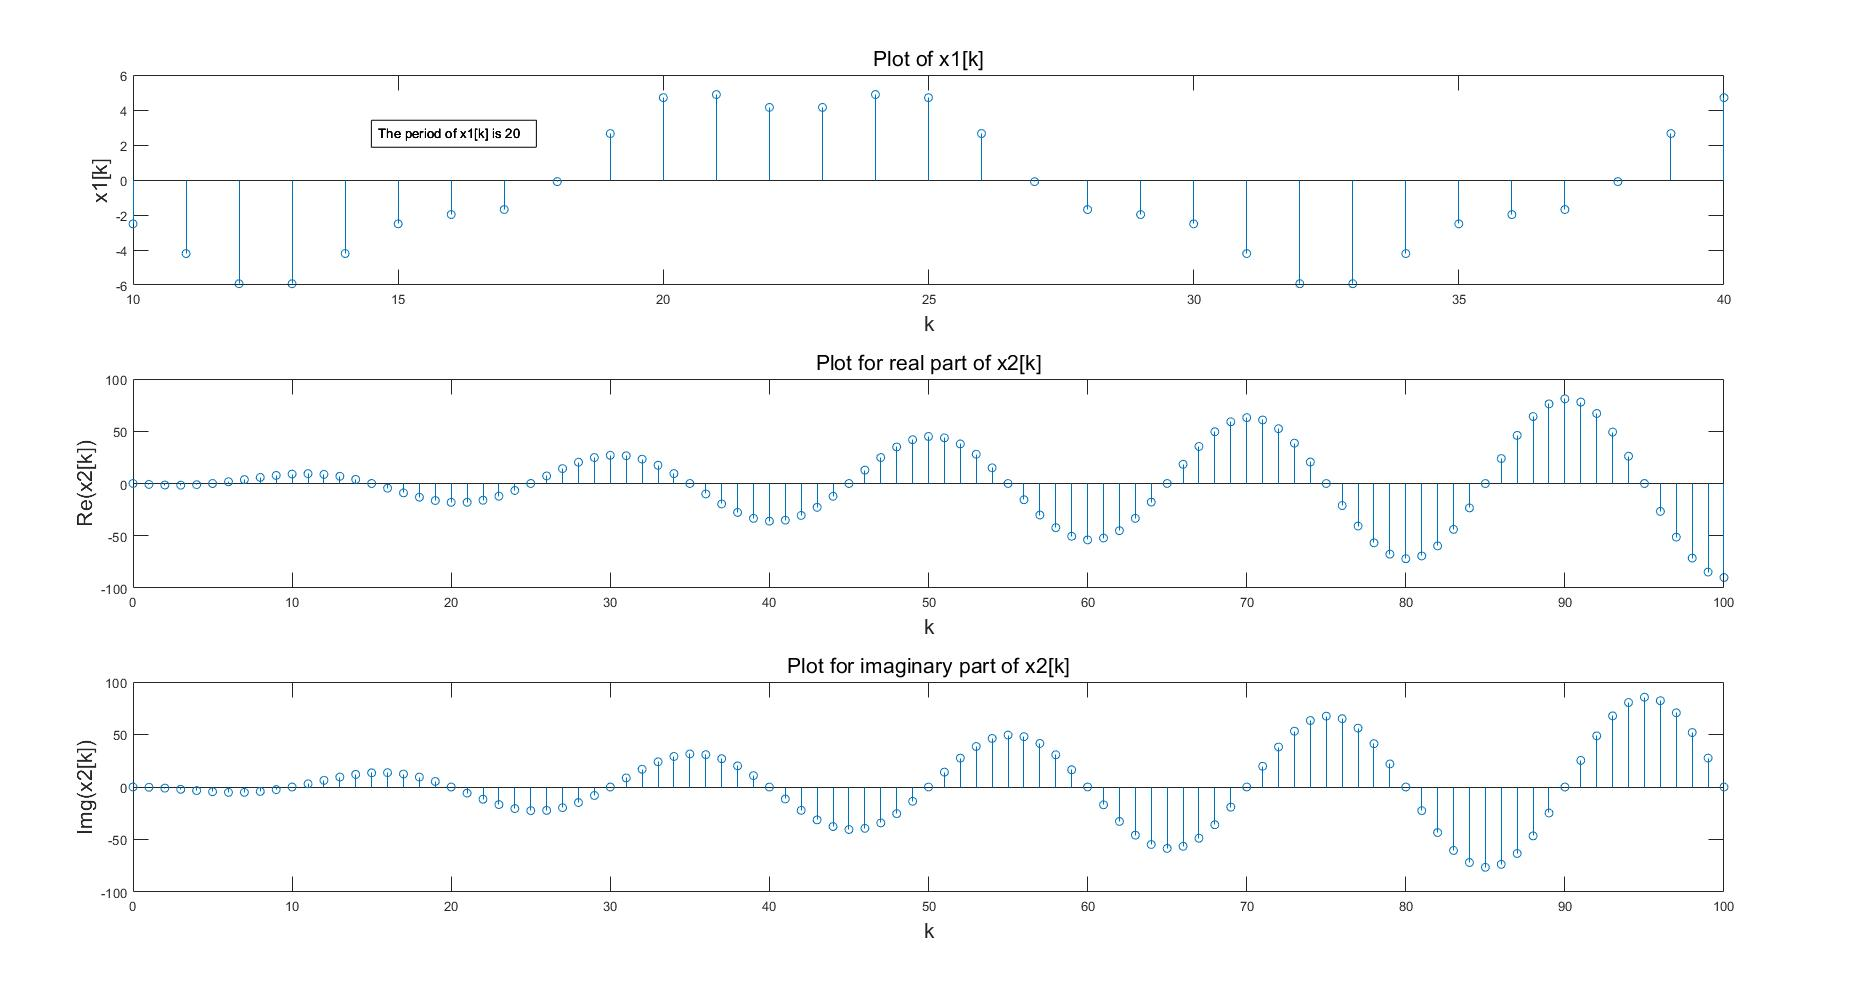
\includegraphics[width=\textwidth]{Q1Plot.jpg}
		
		Associate code for generating the discrete function and plots:
\begin{lstlisting}[language=Matlab]
% initialize input vector for k1 and k2
k1 = (10:40);
k2 = (0:100);

% output vector x1 and x2 with input k1 and k2 respectively
x1 = -5.1 * sin(0.1 * pi * k1 - 3 * pi / 4) + 1.1 * cos(0.4 * pi * k1);
x2 = (-0.9 .* k2) .* exp(1j * pi * k2 / 10);

realX2 = real(x2);  % real part of x2[k]
imagX2 = imag(x2);  % imaginary part of x2[k]

% Set the plot layout. Placing 3 different graph separately in 
% a vertical manner
tiledlayout(3,1);

% plot of x1[k]
ax1 = nexttile;
stem(ax1, k1, x1);
title('Plot of x1[k]', 'Fontsize', 16);
xlabel('k', 'Fontsize', 16);
ylabel('x1[k]', 'Fontsize', 16);
dim = [.2 .78 .1 .1];
text = {'The period of x1[k] is 20'};
annotation('textbox', dim, 'String', text);

% plot of real part of x2[k]
ax2 = nexttile;
stem(ax2, k2, realX2);
title('Plot for real part of x2[k]', 'Fontsize', 16);
xlabel('k', 'Fontsize', 16);
ylabel('Re(x2[k])', 'Fontsize', 16);

% plot of imaginary part of x2[k]
ax3 = nexttile;
stem(ax3, k2, imagX2);
title('Plot for imaginary part of x2[k]', 'Fontsize', 16);
xlabel('k', 'Fontsize', 16);
ylabel('Img(x2[k])', 'Fontsize', 16);
\end{lstlisting}
		
		\item[b)] $x_1[k]$ is a periodic sequence, and period is 20. $x_2[k]$ is not a periodic sequence.
		
		\item[c)] The total energy of $x_1[k]$ is 426.3335. The total energy of $x_2[k]$ is 274063.5.
	\end{enumerate}
	
	\section*{Q.2 Digital Audio}
	\begin{enumerate}
		\item[b)] Code to generate matrix x3:
		
\begin{lstlisting}[language=Matlab]
% Read the audio signal and store it into matrix x3. Fs is the 
% sample rate, which is necessary for write the audio signal 
% into .wav file after processing.
[x3, Fs] = audioread("baila.wav"); 

% A matrix represent the index of each sample.
k = (1:length(x3));
sampleSize = length(x3);  % Size and No. of sample of x3
\end{lstlisting}
		
		\item[c)] The size of $x_3$ matrix is 1000000 x 1.The number of samples is 1000000.
		
		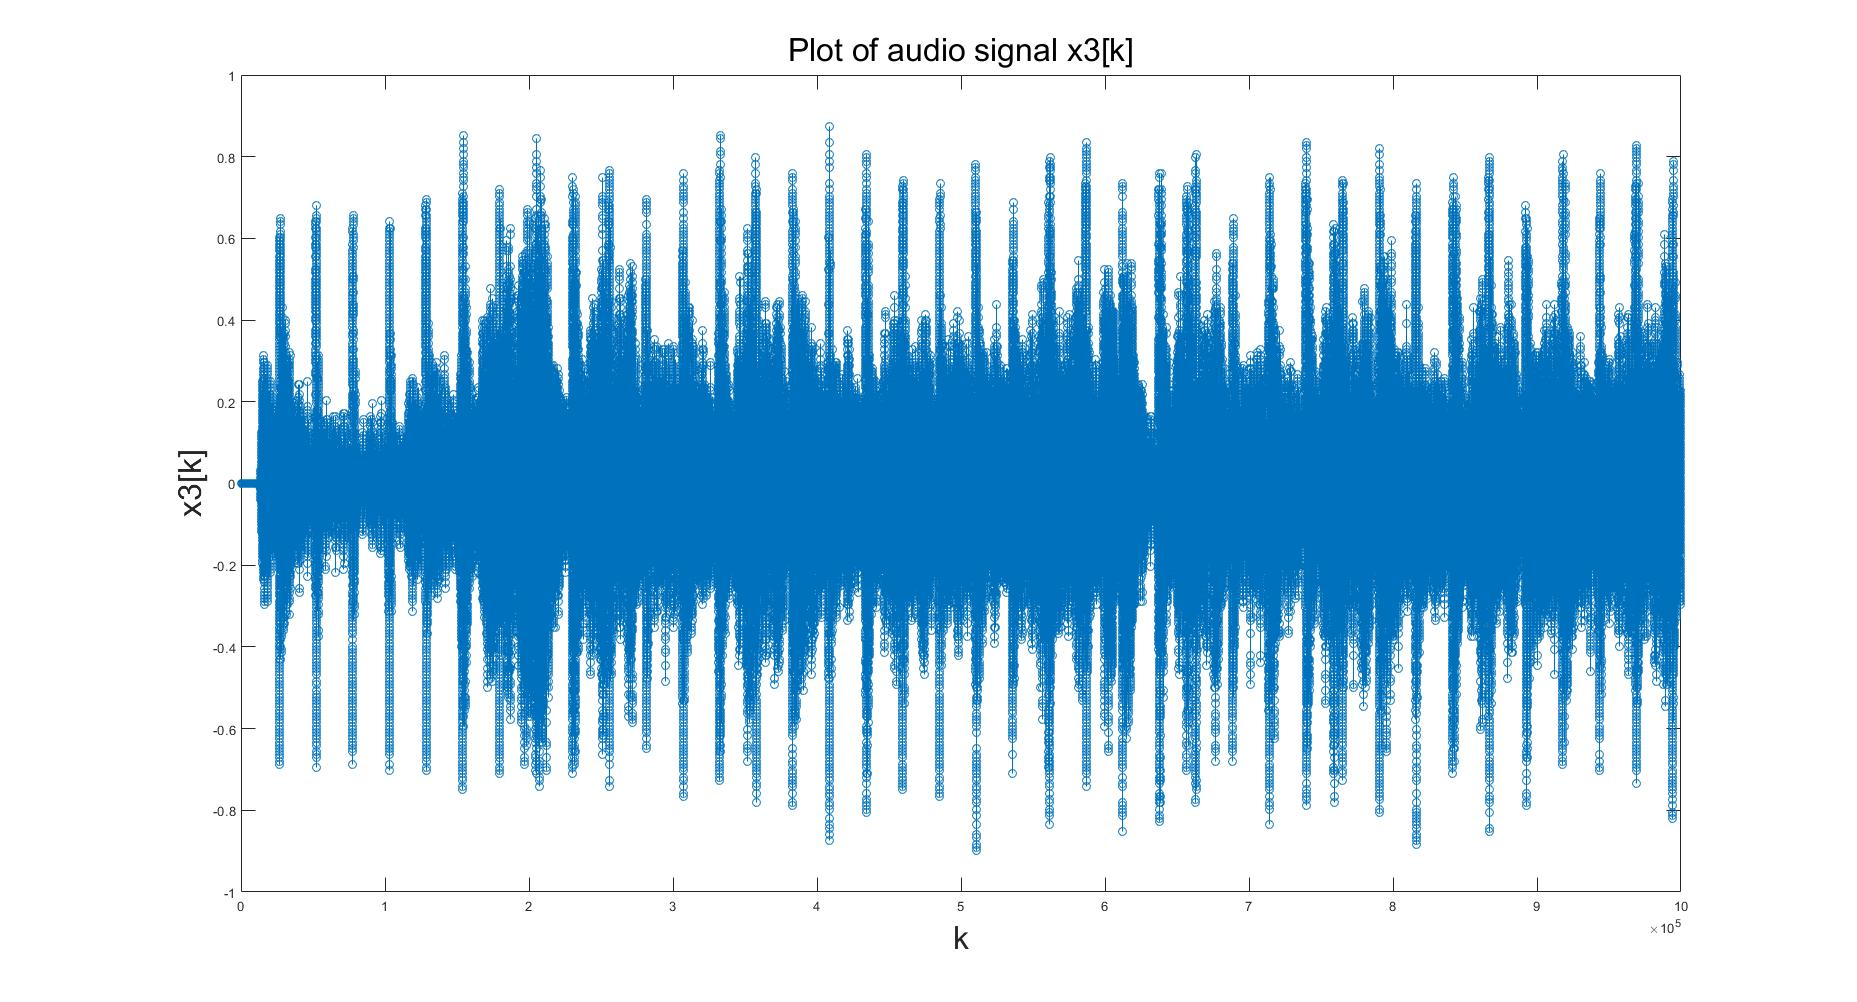
\includegraphics[width=\textwidth]{Q2Plot.jpg}
		
		\item[d)] The energy of $x_3$ is 20422.7731323242.
		
		\item[e)] Code to generated matrix x3s[k]:
		
\begin{lstlisting}[language=Matlab]
% Generate matrix x3s[k] by keeping the first half of x3
x3Half = x3(1:sampleSize/2); 
\end{lstlisting}

		\item[f)] Code for \textbf{baila\_half} file:
		
\begin{lstlisting}[language=Matlab]
% Write x3s[k] into an output audio file.
audiowrite("baila_half.wav", x3Half, Fs);
\end{lstlisting}

	\end{enumerate}

	\section*{Q.3 Digital Image}
	\begin{enumerate}
		\item[b)] No. of both rows and columns are 512. The maximum pixel value is 165.

		Code to store matrix lena:
\begin{lstlisting}[language=Matlab]
lena = imread("lena.jpg"); % Read .jpg file into a matrix
[row, column] = size(lena); % Return the number of row and column
maxPixel = max(max(lena)); % Find the maximum pixel
\end{lstlisting}

		\item[c)] Code for creating \textbf{lena\_bright}:
		
\begin{lstlisting}[language=Matlab]
% Create a brighter version of the .jpg file
lena_bright = lena + 30;
\end{lstlisting}

		\item[d)] Coe for written \textbf{lean\_bright.jpg} file:
\begin{lstlisting}[language=Matlab]
% Write the matrix into a .jpg file
imwrite(lena_bright,'lena_bright.jpg','jpg','Quality', 100);
\end{lstlisting}

	\end{enumerate}

	\section*{Q.4 System response}
	\begin{enumerate}
		\item[a)] The difference equation is $y[k] - ay[k-1] = x[k]$
		\item[b)] 
			\begin{itemize}
				\item Hand Calculation of y[k] for $0 \leq k<5$ and $x[k] = u[k]$
				\begin{itemize}
					\item $a=0.5$
					\begin{align*}
						y[k] &= u[k] + ay[k-1] \\
						k &= 0, y[0] = 1 + 0.5y[-1] = 1 + 0 = 1 \\
						k &= 1, y[0] = 1 + 0.5y[0] = 1 + 0.5 = 1.5 \\
						k &= 2, y[0] = 1 + 0.5y[1] = 1 + 0.75 = 1.75 \\
						k &= 3, y[0] = 1 + 0.5y[2] = 1 + 0.875 = 1.875 \\				
						k &= 4, y[0] = 1 + 0.5y[3] = 1 + 0.9375 = 1.9375 \\				
					\end{align*}
					\item $a=2$
					\begin{align*}
						y[k] &= u[k] + ay[k-1] \\
						k &= 0, y[0] = 1 + 0.5y[-1] = 1 + 0 = 1 \\
						k &= 1, y[0] = 1 + 0.5y[0] = 1 + 2 = 3 \\
						k &= 2, y[0] = 1 + 0.5y[1] = 1 + 6 = 7 \\
						k &= 3, y[0] = 1 + 0.5y[2] = 1 + 14 = 15 \\				
						k &= 4, y[0] = 1 + 0.5y[3] = 1 + 30 = 31 \\					
					\end{align*}
				\end{itemize}
				\item Code Sysresp.m function:
\begin{lstlisting}[language=Matlab]
function y=sysresp(x, a)
% computes the output in response to an arbitrary input 
% x[n], n=0,...N-1
% assume that the system has 0 initial conditions
% input:
% x: the input signal,
% a: the system parameter
% output:
% y: the output signal

% Return the length input signal / input matrix x
n = length(x);

% Initialize the output signal / output matrix y
y = zeros(n, 1); 

% The first sample is always 1 due to given initial 
% condition
y(1) = x(1); 

% Generate each sample from k = 1 to n - 1
for i = 2:n
	y(i) = x(i) + a * y(i-1);
end

return
\end{lstlisting}
				\item When $a = 0.5$, the DT system is BIBO stable. When $a = 2$, the DT
				 system is not BIBO stable because the output signal is not bounded.
				 
				 \item The plot result matches the hand calculation from $0 \leq k<5$. Plot for 
				 $y[k]$ when $a = 0.5$ and $a = 2$:
			\end{itemize}			
		
		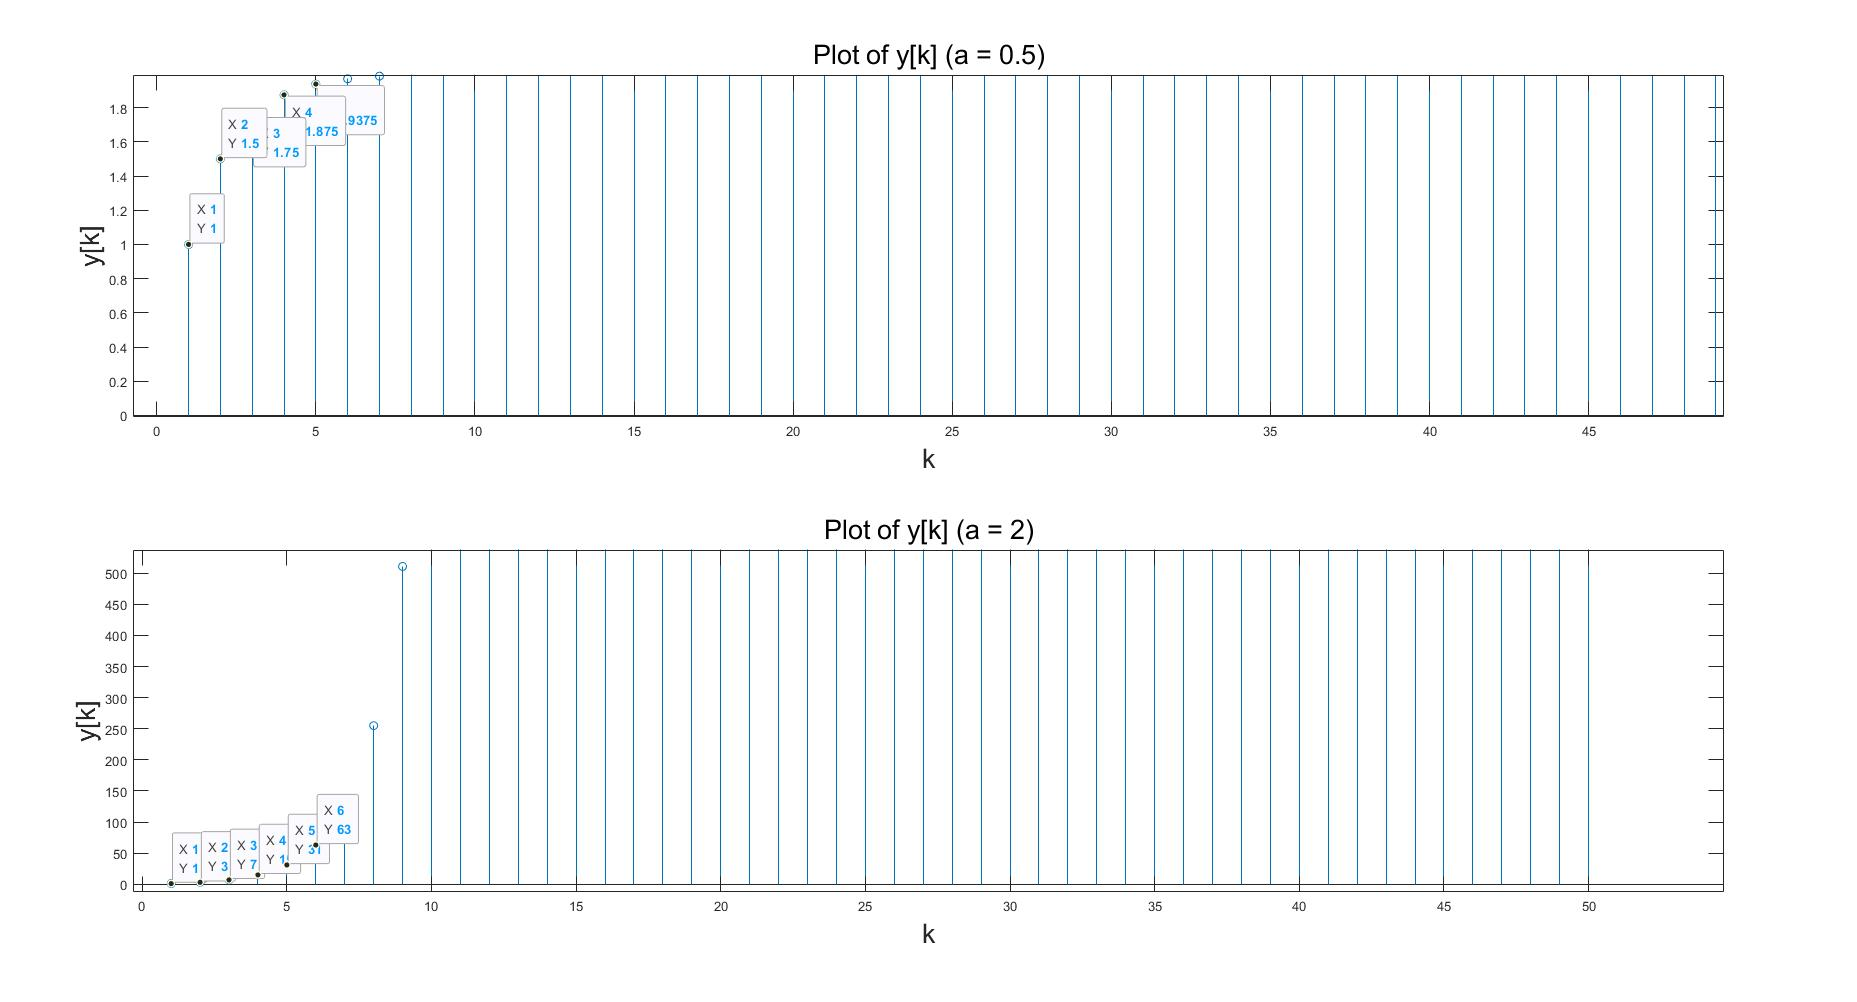
\includegraphics[width=\textwidth]{Q4Plot.jpg}
		
		\item[c)] When a = 0.2, the above system is also BIBO stable. Plot for $y[k]$ when $a=0.2$:
		
		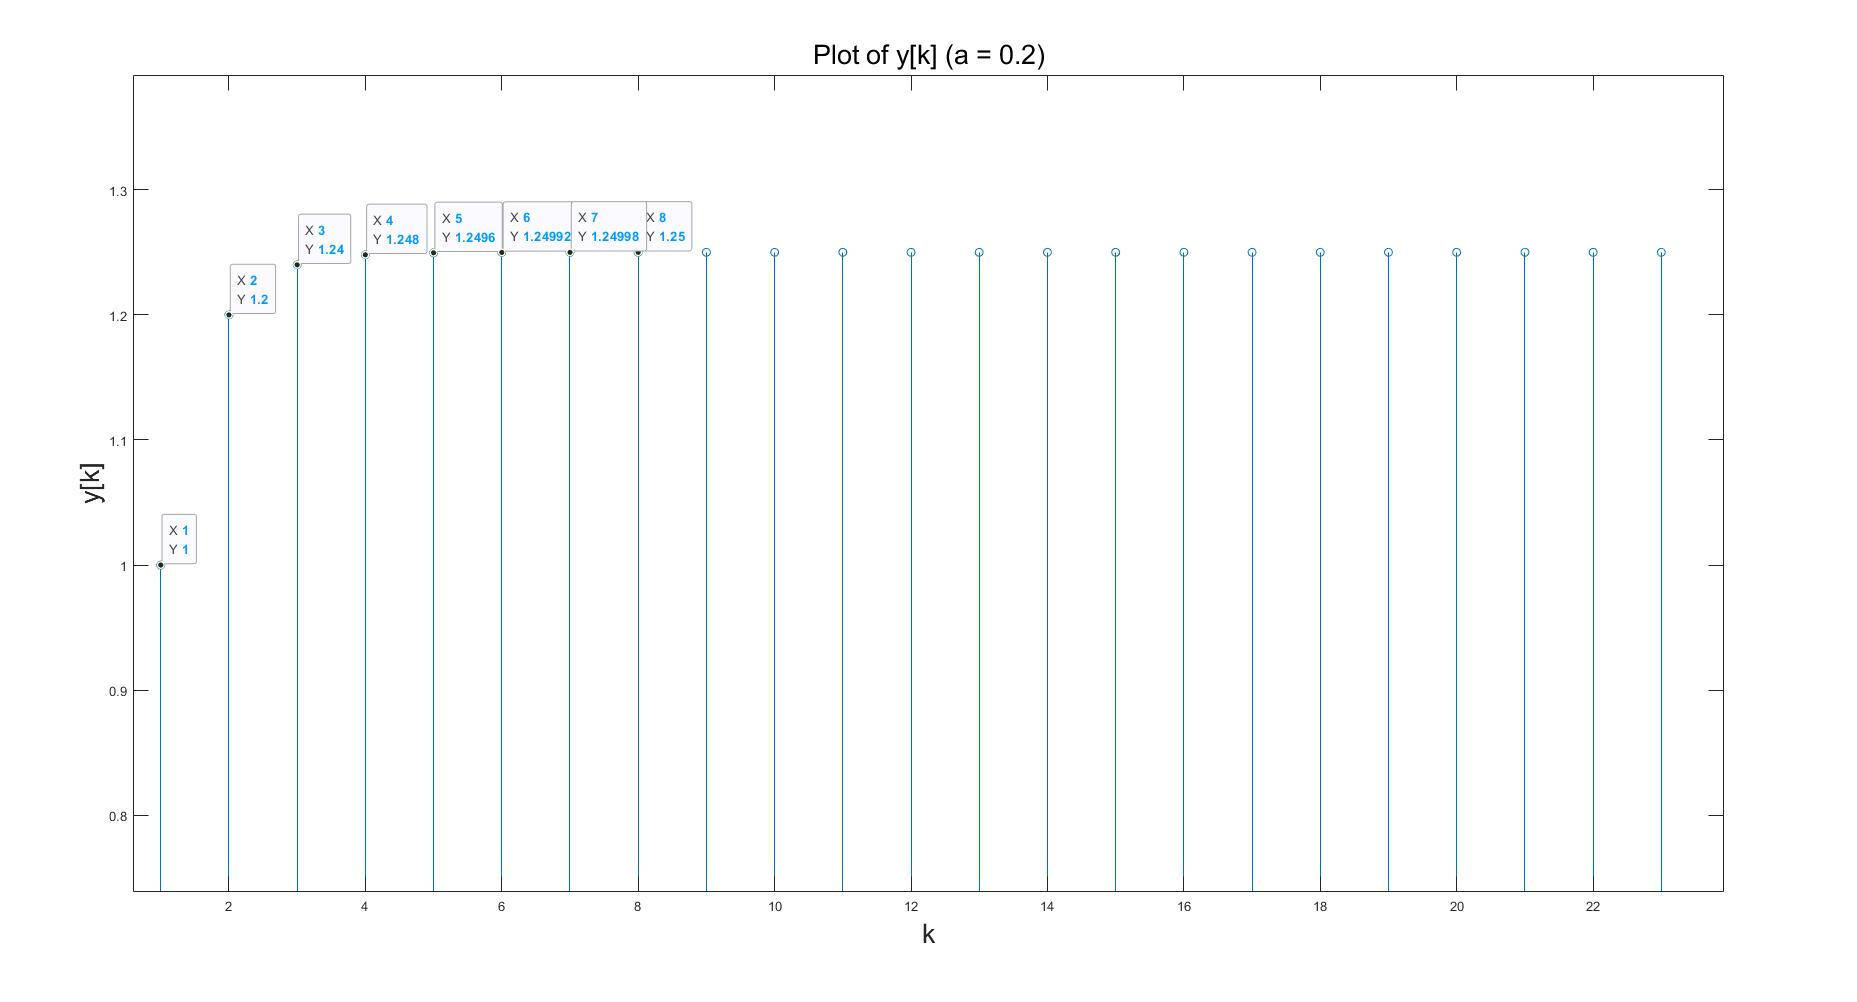
\includegraphics[width=\textwidth]{Q4CPlot.jpg}
	\end{enumerate}

\end{document}